% This is samplepaper.tex, a sample chapter demonstrating the
% LLNCS macro package for Springer Computer Science proceedings;
% Version 2.20 of 2017/10/04
%
\documentclass[runningheads]{llncs}
%
\usepackage[utf8]{inputenc}
\usepackage{graphicx}
\usepackage[british]{babel}
\usepackage{amsmath}
\usepackage[linesnumbered]{algorithm2e}
\usepackage{algorithmic}


%\usepackage[backend=biber]{biblatex}
%\usepackage[backend=biber,style=splncs04]{biblatex}  %backend=biber is 'better'  

% Used for displaying a sample figure. If possible, figure files should
% be included in EPS format.
%
% If you use the hyperref package, please uncomment the following line
% to display URLs in blue roman font according to Springer's eBook style:
% \renewcommand\UrlFont{\color{blue}\rmfamily}

% ---- Bibliography ----
%
% BibTeX users should specify bibliography style 'splncs04'.
% References will then be sorted and formatted in the correct style.
%
\DeclareMathOperator{\sgn}{sgn}


\newcommand{\xn}{\ensuremath{\mathbf{x_0}}}
\newcommand{\rb}{\ensuremath{\mathbf{r}}}
\bibliographystyle{splncs04}
\begin{document}
%
\title{Contribution Title\thanks{Supported by organization x.}}
%
%\titlerunning{Abbreviated paper title}
% If the paper title is too long for the running head, you can set
% an abbreviated paper title here
%
\author{Maurus K\"uhne\inst{1}\orcidID{0000-0002-4205-3552} \and
Beat Tödtli\inst{2}\orcidID{0000-0003-3674-2340}} %\and
%Third Author\inst{3}\orcidID{2222--3333-4444-5555}}
%
\authorrunning{M. Kühne and B.Tödtli}
% First names are abbreviated in the running head.
% If there are more than two authors, 'et al.' is used.
%
\institute{Fernfachhochschule Schweiz\\
\url{ffhs.ch}\and
Institut für Informations- und Prozessmanagement, FHS St.Gallen, \\
\email{beat.toedtli@ost.ch}\\
\url{fhsg.ch} 
}
%
\maketitle              % typeset the header of the contribution
%
\begin{abstract}
The abstract should briefly summarize the contents of the paper in
150--250 words.
\cite{yu_generating_2018}
\keywords{First keyword  \and Second keyword \and Another keyword.}
\end{abstract}
%
%
%

\section{Introduction}
The discovery of Szegedy et.al.~\cite{Szegedy_2014} that several machine learning models including deep neural networks are vulnerable to \emph{adversarial attacks} was seminal for a new subfield of studying deep learning. Probably the most intriguing, but also unsettling result was that adversarial examples can be made quite imperceptible to the human eye, while still fooling a convolutional neural network to misclassify the image~\cite{goodfellow_2014}. Subsequent work has developed various algorithms in a variety of white-box, gray-box and black-box attack scenarios as well as defensive strategies such as adversarial training~\cite{REN2020346}. Moosavi-Dezfooli et. al. have demonstrated that the perturbations can be universal, i.e. that a single set of of pixel modification can be found that fools a network on a large fraction of the training data set~\cite{moosavi-dezfooli_universal_2017}. Moreover, these \emph{universal perturbations} also fool other convolutional networks, albeit to a lesser but still very significant degree~{\bf cite universal adversarial attacks}. 

These results suggest that neural networks partly share a common structure that can be exploited by universal adversarial perturbations (UAP), while yet other aspects are different. Much remains to be understood about the shape of the decision surfaces in neural networks and how they depend on the architecture of the neural network. In this context, we ask whether the transferability of UAP to new convolutional neural networks is improved by combining two neural networks in the adversarial perturbation generation algorithm. By combining two neural networks in the generation process of adversarial examples, one might expect to see an increase in the transferability of an adversarial perturbation to other networks. Ultimately, we hope this approach could lead to identifying a general property resulting in convolutional neural networks being susceptible ({\bf sensitive?} to adversarial attacks.

Given the practical potential and relevance of Deep Learning and the above potential security threats, finding a robust resolution is important and urgent. However, research into the topic is hampered by the \emph{reproducibility crisis} in machine learning~\cite{raff2020quantifying}. A lot of research results, including on adversarial attacks, remain poorly documented in publications. While the methods described may be general enough to be useful for many similar applications, 
the published results are often difficult to reproduce due to undocumented values for hyperparameters, software library versions etc. {\bf ev. https://arxiv.org/vc/arxiv/papers/1909/1909.03032v1.pdf zitieren?}
Also, only in rare cases is it clear how well the published results generalize beyond the very specific data set that was used but not provided to produce the published results. While not being able to reproduce the generation of adversarial examples may seem beneficial at first sight, it is clear that a thorough resolution of such security issues requires a well-stated problem, including readily available state-of-the-art algorithms for the production of adversarial examples. They form the basis of being able to test deep learning systems against such attacks. 

The authors of ~\cite{moosavi-dezfooli_universal_2017} {\bf und weiteren Artikeln, zitieren!} show good generalization results for UAP generated with their procedure \emph{DeepFool}\cite{DeepFool-Moosavi-Dezfooli15} across different deep learning architectures. We report on our reproduction effort, provide our code and investigate whether modifications of DeepFool are able to improve the generalization capability of UAPs. Specifically, we ask whether incorporating information from a second neural network architecture improves the fooling rate of UAPs of a third neural network. We investigate three combination procedures and compare them with the original adversarial attack procedure.

This paper is organized as follows. After an introduction to DeepFool and the construction of UAPs, we describe our reproduction effort of the original work of Moozavi-Dezfooli et.al.~\cite{moosavi-dezfooli_universal_2017}. We then present several modifications of their UAP generation algorithm to construct UAPs that are optimized on two networks. We present our results that compare these variants to the original UAP generation algorithm of Moozavi-Dezfooli et.al. We conclude with a discussion of these results.

\section{Methods}
\subsection{General Setting}
Given a classifier $\hat{k}(x)=\sgn\left(f(x)\right)$ that is based on the sign of a classification function $f:\mathbf{R}^n\rightarrow\mathbf{R}$, adversarial attacks seek a perturbation $v$ such that \[\hat{k}(\mathbf{x}+\mathbf{v})=\sgn\left(f(\mathbf{x}+\mathbf{v})\right)\neq \sgn\left(f(\mathbf{x})\right)=\hat{k}(\mathbf{x}).\] 


\subsection{DeepFool}
In DeepFool, the perturbation $\mathbf{v}$ for an image $\xn$ is defined to be the shortest vector (using the $L_2$-norm $\left\|.\right\|$) such that $\xn+\mathbf{v}$ lies on a decision boundary. 
If $f(x)$ is a linear function $f(x)=\mathbf{w} \mathbf{x}+\mathbf{b}$, then $\mathbf{v}$ can be shown to be $\mathbf{v}=-\frac{f(\xn)}{\left\|\mathbf{w}\right\|_2^2}\mathbf{w}$. As $f$ is nonlinear in general, the Taylor approximation $f(x)=f(\xn)+\left(\nabla f(\mathbf{x})\right)^T\mathbf{v}$ is used to iteratively reach the decision boundary. 
In the multi-class setting considered here, there is an additional step of identifying the closest decision boundary, solved in line 10 of Alg.~\ref{alg:1}.

Perturbations computed at each step are added up and scaled back to satisfy a norm bound given by \(\left\|\mathbf{v}\right\|_2\leq\xi\) where \(\xi\) is a hyperparameter.{\bf stimmt das??} For Details, see~\cite{DeepFool-Moosavi-Dezfooli15}. \\

\begin{figure}
\begin{algorithm}[H]\label{alg:1}
\SetAlgoLined
%\KwResult{Write here the result }
{\bf Input}:image \(\mathbf{x}\), classifier \(f\) with class logits \(f_k\), maximal number of iterations \(i_{\text{max}}\)\;
{\bf Output}: Universal perturbation vector \(\mathbf{\hat{r}}\)\;
Initialize \(\mathbf{x_0} \gets \mathbf{x}\)\;
 \While{\(\hat{k}(\mathbf{x_i}) = \hat{k}(\mathbf{x_0})\) }{
\For { \( i =0\ldots i_\text{max}\)}{

\For { $k \neq \hat{k}(\mathbf{x_0})$ } {
	 ${\mathbf{w'}_k} \gets \nabla f_k(\mathbf{x}) - \nabla f_{\hat{k}(\mathbf{x_0})}(\mathbf{x}) $\;
$f'_k \gets f_k(\mathbf{x}) - f_{\hat{k}(\mathbf{x_0})}(\mathbf{x}) $
}
$\hat{l} \gets \arg \min_{k \neq \hat{k}(\mathbf{x_0})} \frac{ \vert f'_k \vert}{\Vert \mathbf{w'}_k \Vert_2}  $

$\mathbf{r}_i \gets {\frac{\vert f'_{\hat{l}} \vert}{\Vert \mathbf{w'_{\hat{l}}} \Vert^2_2}} \mathbf{w'_{\hat{l}}} $
{\bf	Rescale ???????}\(v\gets \sqrt{\xi}v/\left\|v\right\|_p\)

\(\mathbf{x} \gets \mathbf{x} + \mathbf{r}_i\)\;
}
}
\Return \(\mathbf{\hat{r}}=(1+\eta)\sum_i \mathbf{r}_i\)
 \caption{Multiclass DeepFool}
\end{algorithm}
\end{figure}

\subsection{Universal adversarial Perturbations with DeepFool}
Perturbations generated for each image using DeepFool can be combined to form UAP using Alg.~\ref{alg:2}. To obtain a single UAP for a dataset, DeepFool perturbations of images are added to obtain a universal perturbation (For details, see~\cite{moosavi-dezfooli_universal_2017}). Adding up the perturbations is not commutative, since projections take place once the size (norm) of the perturbation becomes too big {\bf Überprüfen in Algo!}. 
%Intriguingly, although the directions to the class boundaries vary for the training images, the resulting average over all image perturbations does work well, even for other convolutional neural networks. {\bf ALGO Alg.~\ref{alg:2} Hier listen?}

Our main attempt of modifying Alg.~\ref{alg:2} such that it incorporates the weaknesses of several neural networks is to hope for an improvement by incorporating the perturbations obtained for each network individually. In a first attempt, one could simply add up the perturbations stemming from two neural networks. As noted above, because of the norm-projection, this is different from our second attempt (given in Alg.~\ref{alg:3}, in which perturbations for the two networks are added up before projecting onto the norm constraint.

the same universality across different network architectures.
These class boundaries are different
However, when combining several  of identifying the closest class boundary for a given data point. The main cha

We compare this with Algorithm~\ref{alg:3} representing a class of perturbation generating procedures that combine the gradients of several neural networks to construct a single perturbation iteratively. \\

\begin{algorithm}[H]\label{alg:2}

\SetAlgoLined
{\bf Input}:Data set \(X\), classifier \(\hat{k}\), desired norm \(\left\|.\right\|_p\) of
the perturbation \(\xi\), desired accuracy on perturbed samples \(\delta\).\;
{\bf Output}: Universal perturbation vector \(v\)\;
Initialize \(v \gets 0\)\;%, epoch\gets 1\;\;

\While{\textup {Average fooling rate is too low}}{
\ForEach{\(\mathrm{datapoint}\) \(x\in X\) \(\mathrm{with}\) \(\hat{k}(x)=\hat{k}(x+v)\)}{ 
	\(\Delta \rb\gets \underset{r}{\arg \min}\left\|r\right\|_2~\mathrm{s.t.}~\hat{k}(\mathbf{x}+\rb+\Delta\rb)\neq\hat{k}(\mathbf{x})\)\;
	\(\rb\gets \rb+\Delta \rb\)\;  
	\(\rb\gets \sqrt{\xi}\rb/\left\|\rb\right\|_p\)
}  
 }
 \caption{Computation of universal adversarial perturbations}
\end{algorithm}

\begin{figure}
\begin{algorithm}[H]\label{alg:3}
\SetAlgoLined
%\KwResult{Write here the result }
{\bf Input}:image \(\mathbf{x}\), classifier \(f\), maximal number of iterations \(i_{\text{max}}\)\;
{\bf Output}: Universal perturbation vector \(\mathbf{\hat{r}}\)\;
Initialize \(\mathbf{x_0} \gets \mathbf{x}\)\;
 \While{\(\hat{k}(\mathbf{x_i}) = \hat{k}(\mathbf{x_0})\) {\bf and} \( i \leq i_\text{max}\)}{
\ForEach{\(\mathrm{datapoint}\) \(\mathbf{x_0}\in X\) \(\mathrm{with}\) \(\hat{k}(\mathbf{x_0})\neq\hat{k}(\mathbf{x_0}+v)\)}{
\For { $k \neq \hat{k}_f(\mathbf{x_0})$ } {
	 ${\mathbf{w'}_k} \gets \nabla f_k(\mathbf{x}) - \nabla f_{\hat{k}(\mathbf{x_0})}(\mathbf{x}) $\;
$f'_k \gets f_k(\mathbf{x}) - f_{\hat{k}(\mathbf{x_0})}(\mathbf{x}) $
}
\For { $k \neq \hat{k_g}(\mathbf{x_0})$ } {
	 ${\mathbf{u'}_k} \gets \nabla g_k(\mathbf{x}) - \nabla g_{\hat{k}(\mathbf{x_0})}(\mathbf{x}) $\;
$f'_k \gets g_k(\mathbf{x}) - g_{\hat{k}(\mathbf{x_0})}(\mathbf{x}) $
}
$\hat{l} \gets \arg \min_{k \neq \hat{k}(\mathbf{x_0})} \frac{ \vert f'_k \vert}{\Vert \mathbf{w'}_k \Vert_2}  $

$\mathbf{r}_i \gets {\frac{\vert f'_{\hat{l}} \vert}{\Vert \mathbf{w'_{\hat{l}}} \Vert^2_2}} \mathbf{w'_{\hat{l}}} $
{\bf	Rescale ???????}\(v\gets \sqrt{\xi}v/\left\|v\right\|_p\)

\(\mathbf{x} \gets \mathbf{x} + \mathbf{r}_i\)\;
\(i \gets i + 1\)\;
}
}
\Return \(\hat{r}=(1+\eta)\sum_i \mathbf{r}_i\)
 \caption{modified UAP-Generation}
\end{algorithm}
\end{figure}

\subsection{DeepFool and Universal Adversarial Perturbations}
DeepFool~\cite{DeepFool-Moosavi-Dezfooli15} is an algorithm for constructing
- Beschreibung DeepFool
- Beschreibung UAP-Verfahren: Wie werden adv. perturbations von DeepFool zu universal adv. pert. kombiniert
- Beschreibung Kombinationsverfahren: Beschreibe Verfahren ohne modifiziertes DeepFool
\subsection{Results}
\subsubsection{Versuch der Reproduktion Mozavi dezfoli}
		- Resultate Tabelle 7.3. vorstellen und diskutieren:
			- Störwerte und gestörtes Netzwerk identisch 3\%-20\% schlechter als Mozavi
			- gestörtes Netzwerk nicht identisch zum Netzwerk das Störung generiert hat: teilweise bis zu 10\% und 30\% schlechter. 
		- Resultat: Reproduktion sieht qualitativ ähnlich aus. Abb 7.1.
		- ausgeglichenes Datenset; 
		- erwähne, dass Publikation unvollständig für Reproduktion: Defaultwerte von Parameter, welche nicht in publikation beschrieben; Parameterwerte von DeepFool nicht mehr angegeben.
		- Versuch, verschiedene Parameter zu optimieren wurde versucht, brachte nur ca. 5\% Verbesserung
\subsubsection{Kombinationsverfahren}
- Tabelle	8.1 ohne Modifiziertes DeepFool
\begin{table}[]
\centering
\caption{Vergleich der Störraten von einzelnen Störwerten und Kombinationsverfahren (Validation-Set, $l_\infty$, $\xi=10$). Es werden die besten gemessenen Ergebnisse aufgelistet.}
\begin{tabular}{|l|l|l|l|l|l|}
\hline

											&	Inception	&	VGG-16		&	ResNet-152		\\ \hline
Inception-Störwert							&	$81.9\%$		&	$15.9\%$	&	$15.9\%$		\\
VGG-16-Störwert								&	$59.9\%$		&	$58.7\%$	&	$38.0\%$		\\
ResNet-152-Störwert							&	$54.6\%$		&	$31.4\%$	&	$73.4\%$		\\ \hline
lin. Interpolation ($45\% \overline{PQ}$)	&	$46.2\%$		&	$23.7\%$	&	$16.7\%$		\\
Finetuning									&	$59.9\%$		&	$57.9\%$	&	$38.6\%$		\\
abwechselndes Generieren						&	$67.3\%$		&	$60.6\%$	&	$41.2\%$		\\
modifiziertes DeepFool						&	$43.6\%$		&	$18.4\%$	&	$14.1\%$		\\


\hline 
\end{tabular}
\label{tbl_vergleich_comb}
\end{table}
- Diskussion Resultate Reproduktion des UAP-Verfahrens: 
- Diskussion Resultate Kombinationsverfahren: kombiniere Inception und VGG, optimiere Störwerte
Vergleiche mit störwerten, die direkt auf einem einzelnen Modell generiert werden. Vergleiche einerseits mit Störwerten der Einzelmodelle, andererseits mit Störwerten eines unabhängigen Modells (ResNet)

\subsubsection{Discussion}
- Einzelne Parameter konnten nicht gut optimiert werden wegen fehlender Rechenleistung
\subsubsection{Conclusion and Outlook}
Weitere Modellpaare kombinieren.


Lorem ipsum dolor sit amet, consectetur adipiscing elit, sed do eiusmod tempor incididunt ut labore et dolore magna aliqua. Nunc sed augue lacus viverra vitae congue eu consequat. Pellentesque habitant morbi tristique senectus et. Tortor condimentum lacinia quis vel eros donec ac odio tempor. Nibh ipsum consequat nisl vel. Varius sit amet mattis vulputate enim. Ullamcorper eget nulla facilisi etiam dignissim. Sit amet est placerat in. Sed ullamcorper morbi tincidunt ornare massa eget egestas purus. Nibh nisl condimentum id venenatis a condimentum. Quisque sagittis purus sit amet volutpat consequat mauris nunc.

Aliquet risus feugiat in ante metus dictum at. Molestie nunc non blandit massa. Dignissim sodales ut eu sem integer vitae justo. Magna ac placerat vestibulum lectus mauris ultrices eros. Dolor magna eget est lorem ipsum dolor sit amet consectetur. Tincidunt tortor aliquam nulla facilisi cras fermentum odio. Gravida rutrum quisque non tellus orci ac. In vitae turpis massa sed elementum tempus egestas sed. Sit amet luctus venenatis lectus magna fringilla urna. Nibh cras pulvinar mattis nunc sed blandit libero volutpat. Blandit cursus risus at ultrices mi tempus imperdiet nulla malesuada. Non tellus orci ac auctor augue mauris augue neque gravida. Commodo sed egestas egestas fringilla phasellus faucibus scelerisque eleifend. Vitae suscipit tellus mauris a diam.

Pellentesque pulvinar pellentesque habitant morbi tristique senectus. Porttitor lacus luctus accumsan tortor posuere ac ut consequat semper. Velit egestas dui id ornare arcu odio ut sem nulla. Velit laoreet id donec ultrices tincidunt arcu non. Amet purus gravida quis blandit turpis. Malesuada fames ac turpis egestas. Pharetra convallis posuere morbi leo. Proin nibh nisl condimentum id venenatis. Diam vulputate ut pharetra sit amet. Nunc eget lorem dolor sed viverra ipsum nunc aliquet.

Leo vel fringilla est ullamcorper. Integer vitae justo eget magna fermentum iaculis eu. Mi eget mauris pharetra et ultrices. Augue ut lectus arcu bibendum at. Cursus vitae congue mauris rhoncus aenean vel elit scelerisque mauris. Vulputate odio ut enim blandit volutpat maecenas volutpat. Nisi quis eleifend quam adipiscing vitae. Imperdiet dui accumsan sit amet nulla facilisi morbi tempus iaculis. Risus in hendrerit gravida rutrum. Tempus quam pellentesque nec nam aliquam sem. Praesent tristique magna sit amet. Quam viverra orci sagittis eu volutpat odio facilisis. Nunc faucibus a pellentesque sit amet porttitor.

Amet mauris commodo quis imperdiet massa tincidunt nunc pulvinar sapien. Diam sollicitudin tempor id eu nisl nunc mi. Proin fermentum leo vel orci porta non pulvinar. Et molestie ac feugiat sed lectus vestibulum mattis ullamcorper velit. Tincidunt ornare massa eget egestas purus viverra accumsan. Amet est placerat in egestas erat imperdiet sed euismod. Turpis nunc eget lorem dolor. Volutpat sed cras ornare arcu dui vivamus. Turpis massa tincidunt dui ut ornare lectus sit. Etiam tempor orci eu lobortis elementum nibh. Dictumst vestibulum rhoncus est pellentesque elit. Duis at tellus at urna condimentum mattis pellentesque. Sollicitudin aliquam ultrices sagittis orci a scelerisque purus. Nec dui nunc mattis enim ut tellus elementum sagittis vitae. Vulputate mi sit amet mauris commodo quis imperdiet massa tincidunt.


\section{Introduction}
Moozavi-Dezfoli\cite{fawzi_robustness_2017}\\
DeepFool: a simple and accurate method to fool deep neural:\cite{moosavi-dezfooli_deepfool_2016}\\
Universal adversarial perturbations:\cite{moosavi-dezfooli_universal_2017}
\subsection{Results}
Please note that the first paragraph of a section or subsection is
not indented. The first paragraph that follows a table, figure,
equation etc. does not need an indent, either.

Subsequent paragraphs, however, are indented.

\subsubsection{Sample Heading (Third Level)} Only two levels of
headings should be numbered. Lower level headings remain unnumbered;
they are formatted as run-in headings.

\paragraph{Sample Heading (Fourth Level)}
The contribution should contain no more than four levels of
headings. Table~\ref{tab1} gives a summary of all heading levels.

\begin{table}
\caption{Table captions should be placed above the
tables.}\label{tab1}
\begin{tabular}{|l|l|l|}
\hline
Heading level &  Example & Font size and style\\
\hline
Title (centered) &  {\Large\bfseries Lecture Notes} & 14 point, bold\\
1st-level heading &  {\large\bfseries 1 Introduction} & 12 point, bold\\
2nd-level heading & {\bfseries 2.1 Printing Area} & 10 point, bold\\
3rd-level heading & {\bfseries Run-in Heading in Bold.} Text follows & 10 point, bold\\
4th-level heading & {\itshape Lowest Level Heading.} Text follows & 10 point, italic\\
\hline
\end{tabular}
\end{table}

Whenever possible, use vector graphics instead (see
Fig.~\ref{fig1}).

\begin{figure}
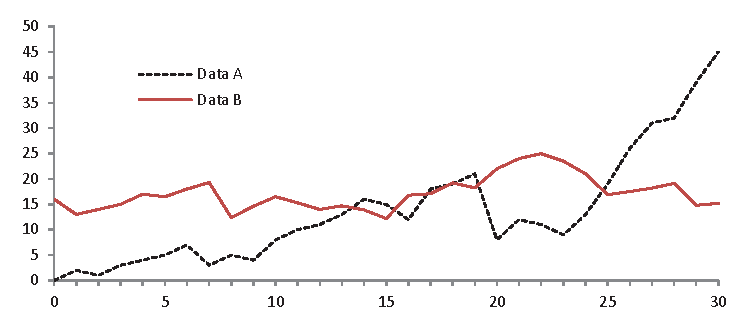
\includegraphics[width=\textwidth]{fig1.eps}
\caption{A figure caption is always placed below the illustration.
Please note that short captions are centered, while long ones are
justified by the macro package automatically.} \label{fig1}
\end{figure}


\bibliography{KuehneToedtli}

\end{document}
We report on an effort to reproduce results from and provide our code. 

- Introduction: adversarial perturbations sind wichtig. 
  Motivation: Vermeidung von Störbarkeit von Netzwerken
	Mozavi dezfoli: es gibt effektive universal adversarial perturbations (auf einer Netzwerkarchitektur trainiert)
	
	Verweis auf noch unbekannte Arbeit
	Fragestellung:
		- Reprodution der Resultate von Mozavi Dezfoli
		- Steigt die Transferierbarkeit von Störwerten, indem ein universal adv. pert verfahren benutzt wird, das mehrere Modelle/Netzwerke kombiniert. 
		- Wir berichten über drei Kombinationsverfahren. und vergleichen diese mit den Resultaten der Originalverfahren.
